\documentclass[a4paper,12pt]{article}
\usepackage{amsmath}
%\usepackage{polish}
\usepackage[polish]{babel}
\usepackage[utf8]{inputenc}
\usepackage[T1]{fontenc}
\usepackage{graphicx}
\usepackage{anysize}
\usepackage{enumerate}
\usepackage{times}
\usepackage{plain}
\usepackage{caption}
\usepackage{graphicx}
\usepackage{setspace}
\usepackage{multirow}
\usepackage{lipsum}
\usepackage{indentfirst}
\usepackage{hyperref}
\hypersetup{
    colorlinks=true,
    linkcolor=blue,
    filecolor=magenta,      
    urlcolor=cyan,
}
\urlstyle{same}
%\marginsize{left}{right}{top}{bottom}
\marginsize{2.5cm}{2.5cm}{2.5cm}{2.5cm}
\setlength{\parindent}{4em}
\setlength{\parskip}{1em}
\renewcommand{\baselinestretch}{2.0}



\begin{document}
\onehalfspacing

\begin{figure}[!htb]
	\centerline{
\includegraphics[scale=0.8]{agh_logo.jpg}}
\end{figure}

\begin{center}
	\Huge{Studio projektowe 1\\}
		\Large{Benchmark solverów prover9 oraz SPASS\\}


	\vspace{5cm}
	\Large{	Autorzy:\\
		Mateusz Grzeliński\\
		Przemysław Michałek\\}

	\newpage

	
\end{center}

\section{Cel}

Celem projektu jest zbadanie wydajności automatyczych metod dowodzenia twierdzeń Prover9 oraz SPASS.

		
\section{Streszczenie}

Badany prover zostaje uruchomiony kilka razy z wcześniej przygotowanym problemem SAT(Boolean satisfiability problem). Badany jest czas wykonywania oraz rezultat (czy SAT jest spełnialny)


\subsection{Prover9}
	Prover9 korzysta z biblioteki \href{https://www.cs.unm.edu/~mccune/prover9/manual/2009-11A/}{LADR} (załączona w źródłach, libladr.a, ladrladr.h). Kompiluje się ona do pliku wykonywalnego.
Prover9 przyjmyje składnie LADR. Konwerter TPTP to LADR jest dostępny w bibliotece LADR

%\newpage

\subsection{SPASS}
	\href{https://webspass.spass-prover.org/}{SPASS} nie korzysta z bibliotek, kompiluje się do pliku wykonywalnego.
Jest duża szansa że można skompilować go do biblioteki. Może korzystać z własnej składni lub ze składni TPTP.
\newpage
\subsection{TPTP}
	\noindent \href{http://www.tptp.org/TPTP/SyntaxBNF.html}{Link do składni BNF} \newline
	\href{http://www.tptp.org/cgi-bin/SeeTPTPCategory=Problems}{Przykład pliku}

TPTP udostępnia wiele problemów do testowania: \href{http://www.tptp.org/cgi-bin/SeeTPTP?Category=Problems}{link} \newline
Te problemy są sklasyfikowane przez domeny (3 literowe skróty), przykładowo \newline
LCL - Logic Calculi \newline
COL - Combinatory Logic

 Pełny opis skrótów dostępny jest \href{http://www.tptp.org/cgi-bin/SeeTPTP?Category=Documents&File=THFSynopsis}{tutaj}
 
\section{Benchmark - strategia blackbox}
Provery traktujemy jako czarne skrzynki, statystyki są ograniczone.\newline
\begin{itemize}
\item TPTP - składnia TPTP
\item LADR - format wejścia Provera9
\item Output - wyjście proverów, mogą być różne
\item statictics - statystyki
\end{itemize}
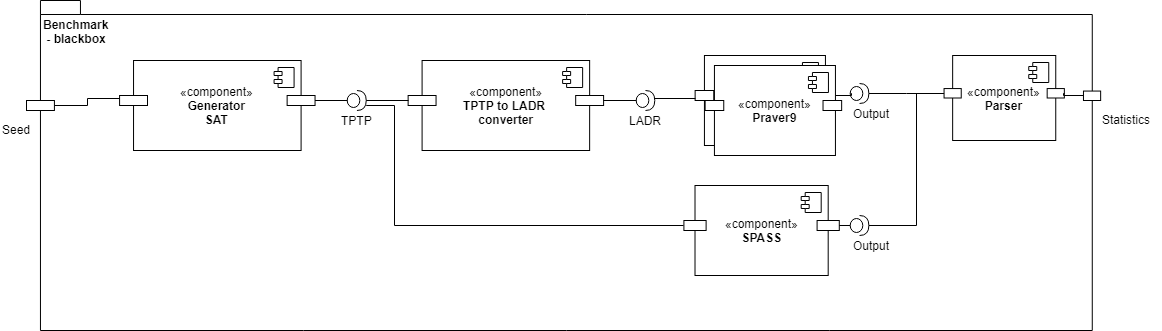
\includegraphics[scale=0.4]{studio-projektowe1.png}
\newpage

\subsection{Algorytm}
\begin{itemize}
\item Wygeneruj formułę SAT
\item Wykonaj kod w podprocesie
\item Zmierz czas wykonania procesu
\item Zbadaj output: dodatkowe statystyki, wynik
\end{itemize}


\section{Generator SAT}
\subsection{Wejście}
\begin{itemize}
\item seed - opcjonalnie - umożliwia powtarzanie losowania
\item typ generatora liczb losowych
\item ilość formuł
\item ilość zmiennych
\end{itemize}


\subsection{Wyjście}
\begin{itemize}
\item string w formacie TPTP (dokumenty do składni: http://www.tptp.org/)
\end{itemize}

\subsection{Algorytm}
\begin{itemize}
\item Wypisz metadane jako komentarz (link do źródła, parametry wejściowe)
\end{itemize}

\newpage
\section{TO DO}
\begin{itemize}
\item czy statystyki czas wykonania, wynik wystarczą? - 
		\begin{itemize}
		\item zaleznosc pomiedzy dlugoscia wejscia a iloscia zmiennych
		\item zajętość pamięci		
		\end{itemize}
		
\item jakie parametry ma przyjmować generator SAT? Czy budujemy generator CNF, czy generator ogólny?
\item  czy brać pod uwagę prametry takie jak
k-SAT, Horn-SAT, NAE3SAT

\item jaki ma być format wyjściowy generatora? 
	\begin{itemize}
		\item propozycja: TPTP - SPASS ma natywne wsparcie dla tego formatu, a prover9 ma translator TPTP to LADR
	\end{itemize}

\item wypisywanie do terminala będzie zabierało czas obliczeń. Trzeba będzie zminimalizować wypisywanie
\item opisać składnie obu proverów

\end{itemize}

\newpage
\section{Słownik}
\noindent
\textbf{SAT} -  problem spełnialności – zagadnienie rachunku zdań, określające czy dla danej formuły logicznej istnieje takie podstawienie (wartościowanie) zmiennych zdaniowych, żeby formuła była prawdziwa \newline
\noindent
\textbf{Prover9} – jest to zautomatyzowane narzędzie udowadniające dla logiki pierwszego rzędu stworzone przez Williama McCune’a \newline
\noindent
\textbf{SPASS} - SPASS Theorem Prover jest narzędziem do automatycznego dowodzenia twierdzeń, należących do rachunku predykatów pierwszego rzędu. \newline
\noindent
\textbf{Logika LTL} – jedna z logik temporalnych. Jest oparta na liniowej strukturze czasu \newline
\noindent
\textbf{Logika temporalna} – logika umożliwiająca rozważanie zależności czasowych bez wprowadzania czasu explicite \newline
\noindent
\textbf{TPTP} (Thousands of Problems for Theorem Provers) - is a library of test problems for automated theorem proving (ATP) systems \newline
\noindent
\textbf{FOF} (First-Order Formula) reduction is a method of attempting to simplify a problem by reducing it to an equivalent set of independent subproblems. A trivial example is to reduce the conjecture A <-> B to the pair of problems A -> B and B -> A.  \newline







\newpage
\section{Wnioski}
\lipsum[1]

\end{document}
